%%%%%%%%%%%%%%%%%%%%%%%%%%%%%%%%%%%%%%%%%%%%%%%%%%%%%%%%%%%%%%%%%%%%%%%%%%%%%%%%%%
\documentclass[12pt]{article}
%%%%%%%%%%%%%%%%%%%%%%%%%%%%%%%%%%%%%%%%%%%%%%%%%%%%%%%%%%%%%%%%%%%%%%%%%%%%%%%%%%
\usepackage{latexsym,amssymb}
%\usepackage[latin1]{inputenc}
%\usepackage{gfsartemisia-euler}
\usepackage[utf8]{inputenc}
\usepackage[spanish,es-nodecimaldot]{babel}
\usepackage{epsfig}
\usepackage{textpos}
\usepackage[utf8]{inputenc}
\usepackage{figlatex}
\usepackage{multirow}
\usepackage{cite}
\usepackage{float}
\usepackage{tikz}
\usepackage{comment}
\usetikzlibrary{arrows.meta, positioning, calc, fit, backgrounds, shadows}
\usepackage{wrapfig} %Inclusi\'{o}n de gr\'{a}ficos al lado de texto
%\usepackage[rflt]{floatflt} %Para meter figuras flotantes entre el texto
\usepackage{hyperref}
\usepackage[version=3]{mhchem} % To write chemical formulae: \ce{H2}
% is easier than $H_2$; another example: Ammonium sulphate is
% written as \ce{(NH4)2SO4}
\usepackage{chemmacros}
\chemsetup{
	formula = chemformula , % or mhchem
	modules = thermodynamics,
	modules = reactions
}
\NewChemState\entropf{
	symbol = S ,
	subscript =f 
}
%\setlength{\oddsidemargin}{0cm}
%\setlength{\evensidemargin}{0cm}
%\setlength{\topmargin}{-1.0cm}
%\setlength{\textwidth}{16.6cm}
%\setlength{\textheight}{21.9cm}
%%%%%%%%%%%%%%%%%%%%%%%%%%%%%%%%%%%%%%%%%%%%%%%%%%%%%%%%%%%%%%%%%%%%%%%%%%%%%%%%%%
\renewcommand{\refname}{Bibliograf\'{i}a}
\renewcommand{\figurename}{Figura}
\newcommand{\kJmol}{$\mathrm{kJ}\cdot\mathrm{mol}^{-1}$}
\newcommand{\rkJmol}{\mathrm{kJ}\cdot\mathrm{mol}^{-1}}
\newcommand{\DHsub}{$\Delta H_{\mathrm{sub}}$}

%%%%%%%%%%%%%%%%%%%%%%%%%%%%%%%%%%%%%%%%%%%%%%%%%%%%%%%%%%%%%%%%%%%%%%%%%%%%%%%%%%
%%%%%%%%%%%%%%%%%%%%%%%%%%%%%%%%%%%%%%%%%%%%%%%%%%%%%%%%%%%%%%%%%%%%%%%%%%%%%%%%%%
\begin{document}
	%%%%%%%%%%%%%%%%%%%%%%%%%%%%%%%%%%%%%%%%%%%%%%%%%%%%%%%%%%%%%%%%%%%%%%%%%%%%%%%%%%
	%%%%%%%%%%%%%%%%%%%%%%%%%%%%%%%%%%%%%%%%%%%%%%%%%%%%%%%%%%%%%%%%%%%%%%%%%%%%%%%%%%
	
	
	\thispagestyle{empty}
	\begin{textblock}{3}(3.5,-2.2)
		
\includegraphics[width=3cm]{buap}
	\end{textblock}
	\begin{textblock}{3}(-0.25,11.5)
		\begin{tabular}{lcr}
			Puebla, Pue. & \phantom{MMMMMMMMMMMMMMMMMM} & Diciembre de 2026
		\end{tabular}
	\end{textblock}
	\phantom{M}
	
	\begin{center}
		\vspace{-1cm}
		\Large\textbf{Benem\'erita Universidad Aut\'onoma de Puebla}
		\vspace{.5cm}
		
		\large Facultad de Ciencias Qu\'{\i}micas y \\
		Centro de Qu\'{\i}mica-Instituto de Ciencias
		
		\vspace{1cm}
		
		Posgrado en Ciencias Qu\'{\i}micas
		\vspace{1.5cm}
		
		\textbf{\LARGE Predictores de $\mathrm{p}K_{\mathrm{a}}$ y $\mathrm{p}K_{\mathrm{b}}$ basados en descriptores qu\'{i}micos y sus isovalores}\\[2em]
		
		\textsc{\large Protocolo de Tesis}\\[0.5em]
		\textsc{\large Doctorado en Ciencias Qu\'{i}micas \\Fisicoqu\'{i}mica }\\[1em]
		\textsc{\large Presenta}\\[1em]
		\textsc{\large M.C. Edgar Garc\'{i}a Ju\'{a}rez}\\[1em]
		
		\normalsize
		
		\vspace{1cm}
		%
		%-----------------------------------------------------
		%
		%Director de Tesis
		%
		%\vspace{1cm}
		%\underline{\phantom{MMMMMMMMMMMMMMMMMM}} \\
		%Dr. Juan Manuel Solano Altamirano
		%
		%-----------------------------------------------------
		%
		\begin{center}
			\begin{tabular}{ccc}
				Director de Tesis &\phantom{M} & Co-director de Tesis \\
				\phantom{M}\\
				\underline{\phantom{MMMMMMMMMMMMMMMM}} & & 	\underline{\phantom{MMMMMMMMMMMMMMMM}}\\
				Dr. Juan Manuel Solano Altamirano & & Dr. Joaqu\'{i}n Barroso Flores
			\end{tabular}
		\end{center}
		%
		%-----------------------------------------------------
	\end{center}
	
	\clearpage
	
	%****************************************************************************
	%section{Resumen}
	%****************************************************************************
	
	
	%****************************************************************************
	\section{Introducci\'{o}n}
	%****************************************************************************
	
	
	%La predicci\'{o}n de los valores de $\mathrm{p}K_{\mathrm{a}}$ y $\mathrm{p}K_{\mathrm{b}}$ son cruciales para comprender la acidez y la basicidad de las mol\'{e}culas org\'{a}nicas, con aplicaciones en el descubrimiento de f\'{a}rmacos, ciencia de los materiales y qu\'{i}mica ambiental. 
	
	Dos de las grandes clasificaciones que existen de los compuestos qu\'{i}micos son en t\'{e}rminos de su acidez o basicidad en sus distintas formulaciones o aceptaciones. El impacto que tienen estas dos clasificaciones en los sistemas vivos es significativo, ya que a un determinado valor de pH ciertos grupos funcionales pueden estar protonados o desprotonados, cuyo fen\'{o}meno est\'{a} relacionado con la constante de  acidez $\mathrm{p}K_{\mathrm{a}}$ que influye, a su vez, en propiedades intr\'{i}nsecas de cada sustancia y cuantifica la fuerza del \'{a}cido en cuesti\'{o}n. La predicci\'{o}n de dicho valor es ampliamente deseable en \'{a}reas como la farmacolog\'{i}a para el desarrollo de nuevos f\'{a}rmacos, o en la bioqu\'{i}mica computacional para el diseño de nuevas prote\'{i}nas.
	Sin embargo, la determinaci\'{o}n experimental del $\mathrm{p}K_{\mathrm{a}}$ y $\mathrm{p}K_{\mathrm{b}}$, mediante t\'{e}cnicas como
	potenciometr\'{i}a, conductimetr\'{i}a, electroforesis, HPLC, UV-vis o 
	fluorometr\'{i}a proporcionan valores con baja precisi\'{o}n (solo las medidas realizadas mediante RMN estiman los valores de $\mathrm{p}K_{\mathrm{a}}$ con precisi\'{o}n cuando se aplica a amino\'{a}cidos) \cite{Haslak2021}.
	
	Por ejemplo, Stivers \textit{et al.} \cite{Stivers1996} midieron valores de 
	$\mathrm{p}K_{\mathrm{a}}$ de los residuos del sitio activo de la 4-oxalocrotonato tautomerasa
	utilizando espectroscop\'{i}a de RMN $^{15}$N. 
	No obstante, los autores reportaron que, para realizar esa medici\'{o}n, se requiere de cristales para un an\'{a}lisis subsecuente mediante cristalograf\'{i}a de rayos X. Desafortunadamente, existe un n\'{u}mero limitado de estructuras de prote\'{i}nas de membrana no soluble presentes en la literatura. Por lo tanto, la pobre resoluci\'{o}n de los cristales y la falta de flexibilidad conformacional restringen las aplicaciones de cristalograf\'{i}a de rayos X y RMN para determinar el $\mathrm{p}K_{\mathrm{a}}$ experimentalmente.
	Respecto a la flexibilidad conformacional, \'{e}sta se debe a la existencia de m\'{u}ltiples 
	especies tautom\'{e}ricas en la reacci\'{o}n general de protonaci\'{o}n-desprotonaci\'{o}n.
	
	En este contexto, el desarrollo de modelos predictivos para determinar el $\mathrm{p}K_{\mathrm{a}}$ resulta fundamental cuando la medici\'{o}n experimental es inviable. Debido a que, estas herramientas permiten estimar dicha propiedad en mol\'{e}culas nuevas. En este sentido, en el presente trabajo se propone diseñar metodolog\'{i}as te\'{o}ricas de bajo costo computacional que permitan calcular dichas constantes.
	
	\clearpage
	
	

	
	%****************************************************************************
	\section{Antecedentes}
	%****************************************************************************
	
	El estudio de los predictores de $\mathrm{p}K_{\mathrm{a}}$ y $\mathrm{p}K_{\mathrm{b}}$ 
	 ha evolucionado a trav\'{e}s de diferentes enfoques con diferentes objetivos. A continuaci\'{o}n,  se muestra una revisi\'{o}n breve del estado del arte de los estudios realizados usando descriptores qu\'{i}micos.
	
	
	En el año de 2019, Caballero-Garc\'{i}a \textit{et al.} \cite{Caballero-Garcia2019} publicaron en el que mejoraron la predicci\'{o}n de la acidez al proponer que el potencial electrost\'{a}tico superficial m\'{a}ximo ($V_{S,max}$) funciona como un descriptor local sensible para el prot\'{o}n \'{a}cido en \'{a}cidos carbox\'{i}licos. En su estudio, analizaron 30 mol\'{e}culas diferentes con valores experimentales de $\mathrm{p}K_{\mathrm{a}}$ reportados en \textit{Handbook of Chemistry} \cite{Lange2005}, encontrando el valor m\'{a}ximo del potencial electrost\'{a}tico sobre la
	isosuperficie de la densidad electr\'{o}nica del hidr\'{o}geno \'{a}cido a 0.001 au.  Es decir, ellos usaron una isosuperficie de densidad y se calcul\'{o} sobre dicha superficie el potencial electrost\'{a}tico, para finalmente obtener el potencial electrost\'{a}tico superficial m\'{a}ximo $V_{S,max}$. Es importante mencionar que el enfoque de Caballero-Garc\'{i}a \textit{et al.} elimin\'{o} la necesidad de calcular la energ\'{i}a libre de solvataci\'{o}n, cuyo procedimiento requiere c\'{a}lculos de alta precisi\'{o}n. Por lo tanto, el modelo presentado por este grupo de investigaci\'{o}n se centr\'{o} en sistemas donde el sitio activo es un grupo hidroxilo, dejando abierta la interrogante sobre su aplicabilidad en bases o sistemas con otros grupos funcionales.
	
	Un año despu\'{e}s de la publicaci\'{o}n anterior, Sandoval-Lira \textit{et al.} \cite{bib:sandovallira2020} complementaron el trabajo de 
	Caballero-Garc\'{i}a \textit{et al.}, al abordar el problema de la basicidad en grupos amino. A diferencia de Caballero-Garc\'{i}a \textit{et al.},
	el grupo de Sandoval-Lira \textit{et al.} identific\'{o} el potencial electrost\'{a}tico m\'{i}nimo ($V_{S,min}$), ubicado en la regi\'{o}n del par 
	electr\'{o}nico no compartido del \'{a}tomo de nitr\'{o}geno, que es un descriptor cr\'{i}tico para determinar el $\mathrm{p}K_{\mathrm{b}}$. 
	Sandoval-Lira \textit{et al.} utilizaron el funcional $\omega$B97X-D, demostrando que es posible predecir 
	el punto isoel\'{e}ctrico ($pI$) de los amino\'{a}cidos al combinar los modelos obtenidos para \'{a}cidos carbox\'{i}licos y grupos amino. 
	Este grupo de investigaci\'{o}n prob\'{o} que la reactividad qu\'{i}mica no solo depende de la mol\'{e}cula analizada, sino también de caracter\'{i}sticas
	 topol\'{o}gicas espec\'{i}ficas (puntos topol\'{o}gicos) en las isosuperficies de potencial. Este hallazgo fundamenta nuestra propuesta de 
	 automatizar la localizaci\'{o}n de dichos puntos adem\'{a}s de la exploraci\'{o}n de nuevos descriptores qu\'{i}micos.
	
	
	
	
	\subsection{Cargas At\'{o}micas y Nuevos Funcionales (2021-2024)}
	
	En el año de 2021, Haslak \textit{et al.} \cite{Haslak2021} se cuestionaron si algunos descriptores qu\'{i}micos que actuan sobre \'{a}tomos de nitr\'{o}geno $Q(N)$ (como energ\'{i}a de ionizaci\'{o}n $I$, afinidad electr\'{o}nica $A$, funciones de Fukui $f+, f-$, entre otras) eran superiores para predecir valores de $\mathrm{p}K_{\mathrm{a}}$ de compuestos derivados de la quinazolina a las cargas at\'{o}micas tradicionales. En su investigaci\'{o}n  probaron 15 conjuntos de bases y 8 funcionales dentro del contexto de la DFT, determinando que las cargas de An\'{a}lisis de Poblaci\'{o}n Natural (NPA), calculadas bajo el modelo de solvataci\'{o}n SMD ofrecen una alternativa computacionalmente econ\'{o}mica para \'{a}cidos carbox\'{i}licos. 
	
	
	El estudio de Haslak \textit{et al.} es relevante para nuestra propuesta, ya que sugiere que el uso de descriptores ``h\'{i}bridos'' (superficie + cargas) podr\'{i}a mejorar la predicci\'{o}n del modelo en sistemas donde la isosuperficie se ve distorsionada por el solvente.
	
	En una l\'{i}nea similar, en el año 2024 Kiran \textit{et al.} \cite{Kiran2024} extendieron el uso de descriptores qu\'{i}micos de la DFT al estudio de derivados de la quinazolina. En este trabajo se introduce la comparaci\'{o}n de nueve descriptores distintos, incluyendo la electrofilicidad, las funciones de Fukui y el descriptor dual. Sus resultados mostraron que, para mol\'{e}culas heteroc\'{i}clicas complejas, no basta con un solo descriptor qu\'{i}mico; la combinaci\'{o}n de la dureza qu\'{i}mica y el potencial qu\'{i}mico mejora la capacidad predictiva. Esto justifica nuestra intenci\'{o}n de no limitarnos solo a la densidad electr\'{o}nica, sino de explorar descriptores qu\'{i}micos como la Funci\'{o}n de Localizaci\'{o}n Electr\'{o}nica (ELF) para identificar zonas de alta localizaci\'{o}n que los modelos de carga simple pasan por alto.
	
	\clearpage
	
	
	\subsection{Sistemas inorg\'{a}nicos y \'{a}cidos ars\'{o}nicos (2025)}
	
	Una posible l\'{i}nea de investigaci\'{o}n de este anteproyecto es la transici\'{o}n hacia sistemas inorg\'{a}nicos, un \'{a}rea abordada recientemente por Nedyalkova \textit{et al.} \cite{Nedyalkova2025}. Su estudio sobre \'{a}cidos ars\'{o}nicos ($RAsO(OH)_2$) es quiz\'{a} el antecedente m\'{a}s directo para nuestra expansi\'{o}n hacia el ars\'{e}nico. Los autores compararon modelos de la DFT con algoritmos de\textit{Support Vector Machine} (SVM), encontrando que el $V_{S,max}$ sigue siendo un descriptor potente para determinar el primer valor de $\mathrm{p}K_{\mathrm{a}}$, pero pierde precisi\'{o}n en la segunda desprotonaci\'{o}n debido a efectos de polarizaci\'{o}n del centro met\'{a}lico. Este trabajo identific\'{o} un punto cr\'{i}tico: los modelos actuales sufren cuando hay una alta diversidad de sustituyentes, lo que refuerza nuestra hip\'{o}tesis de que se requiere explorar m\'{u}ltiples isosuperficies simult\'{a}neamente para capturar la f\'{i}sica del \'{a}tomo de ars\'{e}nico.
	
	\subsection{Machine Learning y el Futuro de la Predicci\'{o}n (2024-2026)}
	
	Actualmente, existe una transformaci\'{o}n en la predicci\'{o}n del $\mathrm{p}K_{\mathrm{a}}$ impulsada por el \textit{machine learning}. Un ejemplo de lo anterior es el trabajo de Rathi \textit{et al.} \cite{Rathi2020}, quienes demostraron que es posible generar superficies de potencial electrost\'{a}tico de alta calidad mediante Redes Neuronales Convolucionales de Grafos (GCNN) en una fracci\'{o}n del tiempo que requieren los c\'{a}lculos de la DFT. Aunque  su enfoque se dirige hacía el diseño de f\'{a}rmacos, la precisi\'{o}n alcanzada sugiere que los descriptores topol\'{o}gicos que planeamos calcular podr\'{i}an, en el futuro, alimentar modelos de entrenamiento masivo. 
	
	Complementario al trabajo anterior, Li \textit{et al.} \cite{Li2024} utilizaron un cribado de alto rendimiento (\textit{High-Throughput Screening}) para predecir la nucleofilicidad de aminas, vinculando directamente c\'{a}lculos de la DFT con modelos \textit{Random Forest}. Este estudio identific\'{o} ``subestructuras cr\'{i}ticas'' que son fragmentos estructurales o grupos de átomos dentro de las moléculas de aminas que ejercen un impacto en el índice de nucleofilicidad y por lo tanto,  influyen en la reactividad en mol\'{e}culas. Un concepto que planeamos aplicar al analizar \'{a}cidos organofosforados. 
	
	\clearpage
	
	Finalmente, el trabajo de Luis-Sim\'{o}n \cite{Simon2026} y Lazare \textit{et al.} \cite{Lazare2025} con la base de datos G-$\mathrm{p}K_{\mathrm{a}}$ y \'{e}steres de \'{a}cidos carbox\'{i}licos (CAE, por sus siglas en ingl\'{e}s) representan la frontera tecnol\'{o}gica, al integrar equilibrios tautom\'{e}ricos conformacionales en el entrenamiento de redes neuronales y herramientas para predecir vida medias de productos org\'{a}nicos detectados en el ambiente. 
	
	
	%La relevancia de este \'{u}ltimo trabajo para nuestro anteproyecto radica en la necesidad de generar datos de alta calidad; nuestra herramienta \texttt{DTK} servir\'{a} como el motor de generaci\'{o}n de descriptores refinados que modelos como los de Luis-Sim\'{o}n requieren para sistemas no org\'{a}nicos.
	
	%+++++++++++++++++++++++++++++++++++++++++++++++++++++++++++++++++++++++
	\subsection{Modelado de constantes de acidez y evaluaci\'{o}n de funcionales}
	%+++++++++++++++++++++++++++++++++++++++++++++++++++++++++++++++++++++++
	
	En el marco de los modelos predictivos para constantes de acidez y basicidad, la elecci\'{o}n del funcional de la densidad (DFT) es cr\'{i}tica para capturar con precisi\'{o}n la topolog\'{i}a electr\'{o}nica. Investigaciones como las de Sandoval-Lira \textit{et al.}\cite{bib:sandovallira2020}, han validado el desempeño del funcional  $\omega$B97X-D, el cual incluye correcciones de dispersi\'{o}n emp\'{i}rica de largo alcance. No obstante, para efectos de este protocolo, se plantea explorar estos resultados con otros funcionales que incorporen de manera expl\'{i}cita correcciones de dispersi\'{o}n (basadas en la aproximaci\'{o}n de Grimme), con el fin de evaluar su impacto en la descripci\'{o}n de las isosuperficies.
	
	Para robustecer y expandir los hallazgos reportados en el estudio  de Sandoval-Lira \textit{et al.} \cite{bib:sandovallira2020} (donde se propone la inclusi\'{o}n de funcionales de reciente implementaci\'{o}n) que no fueron considerados en dicho trabajo, se plantea evaluar el desempeño de funcionales tipo meta-GGA como rSCAN (variantes de la familia SCAN), los cuales podr\'{i}an mostrar una notable precisi\'{o}n en la descripci\'{o}n de enlaces de hidr\'{o}geno y energ\'{i}as de interacci\'{o}n en sistemas moleculares complejos. 
	
	%***************************************************************************
	
	
	\section{Hip\'{o}tesis}
	
	%Es posible encontrar un descriptor de $\mathrm{p}K_{\mathrm{a}}$  a los conocidos a trav\'{e}s de alguna combinaci\'{o}n por determinar de descriptores qu\'{i}micos y sus isovalores.
	
	%La idea principal es: queremos probar varios descritores qu\'{i}micos como isovalores o mejorar la calidad del descriptor (estimador) de pka.
	
	%Es decir, queremos utilizar isosuperficies que no sea de densidad electr\'{i}nica o pensamos que utilizar isosuperfices que no sean de densidad electr\'{o}nica podr\'{}ian mejorarse los descriptores qu\'{i}micos.
	
	Es posible mejorar la calidad de los actuales descriptores de $\mathrm{p}K_{\mathrm{a}}$ y $\mathrm{p}K_{\mathrm{b}}$ mediante el uso de descriptores qu\'{i}micos evaluados sobre distintas isosuperficies a la densidad electr\'{o}nica convencional. La exploraci\'{o}n de diversas funciones de contorno y sus isovalores asociados permitir\'{a} definir un estimador multivariado con mayor capacidad de correlaci\'{o}n que los modelos actuales.
	
	\clearpage
	
	
	%****************************************************************************
	\section{Objetivos}
	%****************************************************************************
	%+++++++++++++++++++++++++++++++++++++++++++++++++++++++++++++++++++++++
	\subsection{Objetivo general}
	%+++++++++++++++++++++++++++++++++++++++++++++++++++++++++++++++++++++++
	%Desarrollar una metodolog\'{i}a  a partir del c\'{a}lculo y mapeo de descriptores fisicoqu\'{i}micos a distintos isovalores a partir de otros descriptores qu\'{i}micos con el fin de establecer un modelo matem\'{a}tico preciso para la predicci\'{o}n de valores de $\mathrm{p}K_{\mathrm{a}}$ y $\mathrm{p}K_{\mathrm{b}}$ en mol\'{e}culas de inter\'{e}s.
	
	
	Desarrollar una metodolog\'{i}a  basada en descriptores qu\'{i}micos 
	para mejorar la predicci\'{o}n de $\mathrm{p}K_{\mathrm{a}}$ y $\mathrm{p}K_{\mathrm{b}}$ en mol\'{e}culas de inter\'{e}s. Se buscar\'{a} la mejor combinaci\'{o}n de descriptores que mapeados sobre diferentes isosuperficies genere los mejores resultados.
	
	
	
	%+++++++++++++++++++++++++++++++++++++++++++++++++++++++++++++++++++++++
	\subsection{ Objetivos espec\'{i}ficos}
	%+++++++++++++++++++++++++++++++++++++++++++++++++++++++++++++++++++++++
	\begin{enumerate}
	
		\item Realizar un an\'{a}lisis exhaustivo de \'{a}cidos org\'{a}nicos pr\'{o}ticos convencionales (carbox\'{i}licos, fen\'{o}licos y \'{e}steres) y otros derivados para crear una base de conocimiento robusta que sirva como gu\'{i}a interpretativa en la caracterizaci\'{o}n de sistemas inorg\'{a}nicos complejos.
		
		
		\item Verificar si la inclusi\'{o}n de dispersi\'{o}n en la contribuci\'{o}n de intercambio y correlaci\'{o}n del funcional mejora la correlaci\'{o}n entre  $V_{S,min}$ y $V_{S,max}$ con los valores experimentales de  $\mathrm{p}K_{\mathrm{a}}$ y $\mathrm{p}K_{\mathrm{b}}$, respectivamente.
		
		%\item Determinar la sensibilidad de los descriptores qu\'{i}micos frente a la contribuci\'{o}n de intercambio y correlaci\'{o}n de funcionales que no dependen de par\'{a}metros ajustados emp\'{i}ricamente para sistemas espec\'{i}ficos.
		
		\item Analizar el uso de isosuperficies alternativas a la densidad electr\'{o}nica para mejorar la precisi\'{o}n de los descriptores qu\'{i}micos y la predicci\'{o}n del 
		$\mathrm{p}K_{\mathrm{a}}$ y $\mathrm{p}K_{\mathrm{b}}$.
		
		%La idea principal es: queremos probar varios descritores qu\'{i}micos como isovalores o mejorar la calidad del descriptor (estimador) de pka.
		
		%Es decir, queremos utilizar isosuperficies que no sea de densidad electr\'{i}nica o pensamos que utilizar isosuperfices que no sean de densidad electr\'{o}nica podr\'{i}an mejorarse los descritores qu\'{i}micos.
		
		
		%\item Expandir el conocimiento sobre la influencia de los orbitales de alta energ\'{i}a en sistemas organofosforados y ars\'{o}nicos bajo marcos te\'{o}ricos m\'{a}s rigurosos.
		
		
		%Los puntos anteriores se basan en la caracterizaci\'{o}n de centros b\'{a}sicos y \'{a}cidos mediante descriptores de superficie a partir de los siguientes puntos:
		
		\item 
		%Expansi\'{o}n de la metodolog\'{i}a a sistemas organofosforados de relevancia biol\'{o}gica
		Ampliar el marco de estudio de mol\'{e}culas org\'{a}nicas convencionales (H, C, N, O) hacia \'{a}cidos organofosforados, profundizando en los efectos de orbitales de alta energ\'{i}a en ausencia de hiperconjugaci\'{o}n, dada su trascendencia en procesos metab\'{o}licos y bioenerg\'{e}ticos.
		
		\item Modelado de acidez en sistemas de ars\'{e}nico: Evaluar los valores de $\mathrm{p}K_{\mathrm{a}}$ en \'{a}cidos ars\'{o}nicos, 
		reportado por Nedyalkova \textit{et al.} \cite{Nedyalkova2025}, considerando su comportamiento en medios acuosos. 
		%El estudio se centrar\'{a} en la respuesta de los descriptores locales frente a cambios en el entorno hidrof\'{o}bico/hidrof\'{i}lico de la mol\'{e}cula de inter\'{e}s.
		
		
		%\item \textit{Alternativo al item anterior}. Evaluar el comportamiento de descriptores fisicoqu\'{i}micos en \'{a}cidos org\'{a}nicos comunes para establecer una base de conocimiento que sirva como modelo de referencia en la caracterizaci\'{o}n de sistemas inorg\'{a}nicos.
		
		%\item Caracterizar el $V_{S,min}$ en la vecindad del par electr\'{o}nico no compartido del \'{a}tomo de nitr\'{o}geno para predecir la basicidad en aminas.
		%\item Desarrollar un protocolo de c\'{a}lculo de  $\mathrm{p}K_{\mathrm{a}}$ para \'{a}cidos ars\'{o}nicos con precisi\'{o}n adaptable a su grado de solubilidad.
		%\item Investigar la influencia de la configuraci\'{o}n electr\'{o}nica y la topolog\'{i}a de isosuperficies en \'{a}cidos organofosforados, excluyendo efectos de deslocalizaci\'{o}n hiperconjugativa.
		
	\end{enumerate}
	
	
	
	
	%Comentar que se tienen todas los wfxs.
	
	%Utilizar diferentes conf\'{o}rmeros y utilizar promedios ponderados.
	
	\clearpage
	
	%****************************************************************************
	\section{Metodolog\'{i}a}
	%****************************************************************************
	
		Actualmente, la determinaci\'{o}n de propiedades moleculares mediante el an\'{a}lisis de isosuperficies presenta limitaciones en t\'{e}rminos de la diversidad metodol\'{o}gica de descriptores que existen. 
	Por lo tanto, es necesario desarrollar estrategias que integren m\'{u}ltiples funciones de localizaci\'{o}n electr\'{o}nica y potenciales electrost\'{a}ticos para mejorar la predicci\'{o}n en sistemas qu\'{i}micos complejos. Debido a lo anterior, nuestra propuesta se fundamenta en los siguientes puntos, que se muestran en la Figura \ref{fig:metodologia_pka}. 

	\begin{itemize}
		
		\item \textbf{Grupos de entrenamiento y prueba}: Seleccionar un conjunto de valores de $\mathrm{p}K_{\mathrm{a}}$ y $\mathrm{p}K_{\mathrm{b}}$ de mol\'{e}culas para establecer grupos de entrenamiento y prueba en un modelo.
	
		
		\item \textbf{An\'{a}lisis de centros nucleof\'{i}licos en aminas:} Determinaci\'{o}n cuantitativa del potencial electrost\'{a}tico m\'{i}nimo superficial ($V_{S,min}$) asociado a los pares solitarios del \'{a}tomo de nitr\'{o}geno. Se tomar\'{a} como referencia la metodolog\'{i}a reportada en la literatura reciente por Haslak \textit{et al.} \cite{Haslak2021} para isosuperficies centradas en el \'{a}tomo de nitr\'{o}geno, estableciendo una correlaci\'{o}n directa con los valores de $\mathrm{p}K_{\mathrm{b}}$ de diversas aminas.
		
		\item \textbf{Automatizaci\'{o}n y escalabilidad:} Implementaci\'{o}n del entorno (el entorno corresponde a la herramienta computacional que permite automatizar el postprocesamiento de datos, como el c\'{a}lculo de isovalores y la evaluaci\'{o}n de descriptores en superficies de contorno de forma sistem\'{a}tica y escalable) en un software propio para optimizar el c\'{a}lculo de isovalores, reduciendo los tiempos de c\'{o}mputo en comparaci\'{o}n con las metodolog\'{i}as tradicionales.
		
		\item \textbf{An\'{a}lisis multidimensional de isosuperficies:} Extender el an\'{a}lisis de la densidad electr\'{o}nica convencional incluyendo algunos (e idealmente todos) de los siguientes descriptores: Funci\'{o}n de Localizaci\'{o}n Electr\'{o}nica (ELF), Potencial Electrost\'{a}tico Molecular (MEP), Regi\'{o}n de Electrones Lentos (ROSE), Gradiente Reducido de Densidad (RDG), Localizador de Orbitales Localizados (LOL), sobre diversas superficies de contorno.
		
		\clearpage
		
		\item \textbf{Modelado predictivo de $\mathrm{p}K_{\mathrm{a}}$:} Desarrollar una expresi\'{o}n matem\'{a}tica que se correlacione, donde el $\mathrm{p}K_{\mathrm{a}}$ se defina como una funci\'{o}n dependiente de los descriptores fisicoqu\'{i}micos y otros par\'{a}metros de isovalores seleccionados, v\'{e}ase la ecuaci\'{o}n \ref{eq:pkaiso}.
		\begin{equation}
			pK_a = f(\text{descriptores, isovalores})
			\label{eq:pkaiso}
		\end{equation}
	\end{itemize}
	
	\begin{figure}[H]
		\centering
		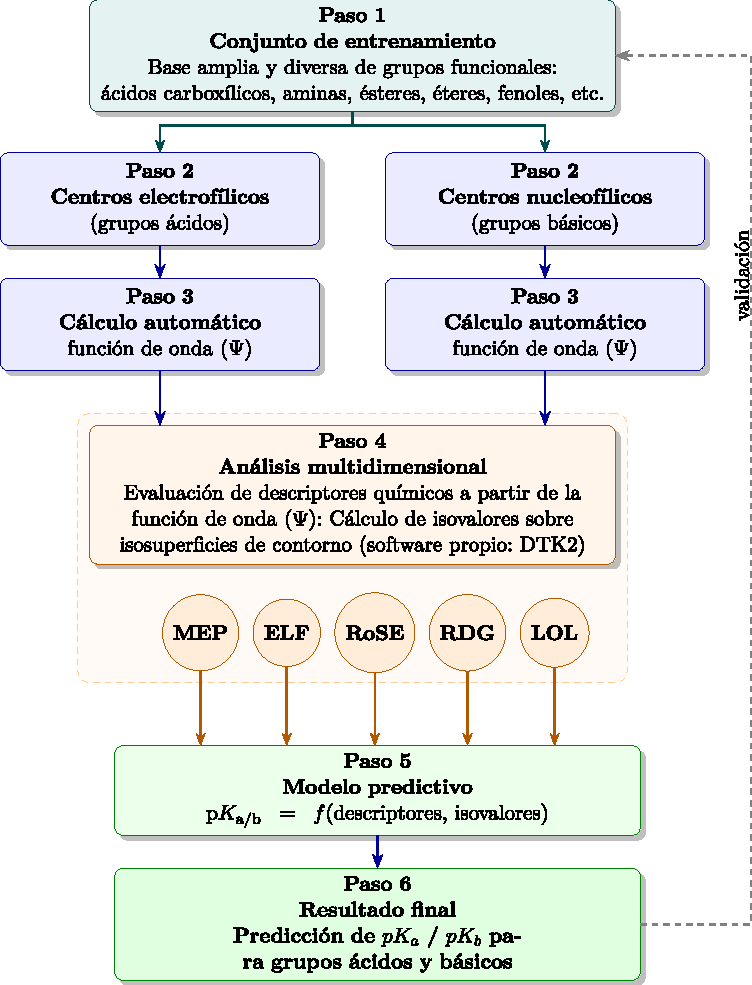
\includegraphics[width=0.8\linewidth]{graphs/metodologia}
		\caption{Metodolog\'{i}a para la predicci\'{o}n de valores de $\mathrm{p}K_{\mathrm{a}}$ y  $\mathrm{p}K_{\mathrm{b}}$  mediante descriptores qu\'{i}micos basados en la densidad electr\'{o}nica.}
		\label{fig:metodologia_pka}
	\end{figure}
	
	
	\begin{comment}
		\begin{figure}[htbp]
		\centering
		% Si el diagrama queda muy grande para tu p\'{a}gina, puedes descomentar la siguiente l\'{i}nea:
		%\resizebox{0.9\textwidth}{!}{%
			\begin{tikzpicture}[
				node distance=0.6cm and 1.2cm,
				etapa/.style={
					rectangle, rounded corners=4pt,
					draw=blue!60!black, fill=blue!8,
					text width=5.6cm, align=center,
					minimum height=1.7cm, font=\small,
					drop shadow
				},
				etapaAncha/.style={
					rectangle, rounded corners=4pt,
					draw=blue!60!black, fill=blue!8,
					text width=9.4cm, align=center,
					minimum height=1.3cm, font=\small,
					drop shadow
				},
				etapaNaranja/.style={
					rectangle, rounded corners=4pt,
					draw=orange!70!black, fill=orange!8,
					text width=9.4cm, align=center,
					minimum height=1.5cm, font=\small,
					drop shadow
				},
				etapaVerde/.style={
					rectangle, rounded corners=4pt,
					draw=green!50!black, fill=green!8,
					text width=9.4cm, align=center,
					minimum height=1.3cm, font=\small,
					drop shadow
				},
				descriptor/.style={
					circle, draw=orange!70!black, fill=orange!15,
					minimum size=0.95cm, font=\small\bfseries
				},
				resultado/.style={
					rectangle, rounded corners=4pt,
					draw=green!50!black, fill=green!12,
					text width=9.4cm, align=center,
					minimum height=1.2cm, font=\small\bfseries,
					drop shadow
				},
				flecha/.style={-{Stealth[length=2.5mm]}, thick, blue!60!black},
				flechadesc/.style={-{Stealth[length=2.2mm]}, thick, orange!70!black},
				flechagrupo/.style={-{Stealth[length=2.2mm]}, thick, teal!60!black}
				]
				
				% ============================================================
				% PASO 1
				% ============================================================
				\node[etapaAncha, fill=teal!10, draw=teal!60!black] (e1) {
					\textbf{Paso 1 \\ Conjunto de entrenamiento}\\
					Base amplia y diversa de grupos funcionales: \\ \'{a}cidos carbox\'{i}licos, aminas, \'{e}steres, \'{e}teres, fenoles, etc.
				};
				
				% ============================================================
				% PASO 2
				% ============================================================
				\node[etapa, below left=0.75cm and 0.6cm of e1.south] (e2a) {
					\textbf{Paso 2 \\ Centros electrof\'{i}licos}\\
					(grupos \'{a}cidos)
				};
				\node[etapa, below right=0.75cm and 0.6cm of e1.south] (e2b) {
					\textbf{Paso 2 \\ Centros nucleof\'{i}licos}\\
					(grupos b\'{a}sicos)
				};
				\draw[flechagrupo] (e1.south) -- ++(0,-0.25) -| (e2a.north);
				\draw[flechagrupo] (e1.south) -- ++(0,-0.25) -| (e2b.north);
				
				% ============================================================
				% PASO 3
				% ============================================================
				\node[etapa, below=0.6cm of e2a] (e3a) {
					\textbf{Paso 3 \\ C\'{a}lculo autom\'{a}tico}\\
					funci\'{o}n de onda ($\Psi$)
				};
				\node[etapa, below=0.6cm of e2b] (e3b) {
					\textbf{Paso 3 \\ C\'{a}lculo autom\'{a}tico}\\
					funci\'{o}n de onda ($\Psi$) 
				};
				\draw[flecha] (e2a) -- (e3a);
				\draw[flecha] (e2b) -- (e3b);
				
				% ============================================================
				% PASO 4
				% ============================================================
				\node[etapaNaranja, below=1.0cm of $(e3a.south)!0.5!(e3b.south)$] (e4) {
					\textbf{Paso 4 \\ An\'{a}lisis multidimensional}\\
					Evaluaci\'{o}n de descriptores qu\'{i}micos a partir de la funci\'{o}n de onda ($\Psi$): C\'{a}lculo de isovalores sobre isosuperficies de contorno (software propio: DTK2) 
				};
				
				\draw[flecha] (e3a.south) -- (e3a.south |- e4.north);
				\draw[flecha] (e3b.south) -- (e3b.south |- e4.north);
				
				% ============================================================
				% Descriptores
				% ============================================================
				\node[descriptor, below=0.55cm of e4.south, xshift=-2.8cm] (mep) {MEP};
				\node[descriptor, right=0.25cm of mep] (elf) {ELF};
				\node[descriptor, right=0.25cm of elf] (rose) {RoSE};
				\node[descriptor, right=0.25cm of rose] (rdg) {RDG};
				\node[descriptor, right=0.25cm of rdg] (lol) {LOL};
				
				% ============================================================
				% PASO 5
				% ============================================================
				\node[etapaVerde, below=1.4cm of $(mep.south)!0.5!(lol.south)$] (e5) {
					\textbf{Paso 5 \\  Modelo predictivo}\\
					$\mathrm{p}K_{\mathrm{a/b}} = f(\text{descriptores},\, \text{isovalores})$
				};
				
				\foreach \d in {mep, elf, rose, rdg, lol} {
					\draw[flechadesc] (\d.south) -- (\d.south |- e5.north);
				}
				
				% ============================================================
				% PASO 6
				% ============================================================
				\node[resultado, below=0.6cm of e5] (e6) {
					\textbf{Paso 6 \\ Resultado final}\\
					Predicci\'{o}n de $pK_a$ / $pK_b$ para grupos \'{a}cidos y b\'{a}sicos
				};
				\draw[flecha] (e5) -- (e6);
				
				% ============================================================
				% Retroalimentaci\'{o}n — canal a la derecha + etiqueta exterior
				% ============================================================
				\coordinate (rightbound) at ([xshift=2.5cm]e4.east);
				\draw[flecha, dashed, gray]
				(e6.east) -- (e6.east -| rightbound)
				-- (e1.east -| rightbound)
				-- (e1.east);
				
				% Etiqueta FUERA de la l\'{i}nea, a la derecha del canal, tamaño \small y rotada
				\node[font=\small, text=black, rotate=90, anchor=south, inner sep=1pt]
				at ($(e4.east -| rightbound)!0.5!(e1.east -| rightbound)$) {validaci\'{o}n};
				
				% ============================================================
				% Reserva de espacio a la derecha para evitar recortes
				% ============================================================
				\path (e4.east -| rightbound) ++(1.2cm,0);
				
				% ============================================================
				% Fondo del bloque Paso 4 + descriptores
				% ============================================================
				\begin{scope}[on background layer]
					\node[fit=(e4)(mep)(lol), fill=orange!4, rounded corners=6pt, inner sep=6pt,
					draw=orange!40, dashed] {};
				\end{scope}
				
			\end{tikzpicture}
			%} % <--- Descomenta tambi\'{e}n esta llave si usas \resizebox arriba
		\caption{Metodolog\'{i}a para la predicci\'{o}n de valores de $\mathrm{p}K_{\mathrm{a}}$ y  $\mathrm{p}K_{\mathrm{b}}$  mediante descriptores qu\'{i}micos basados en la densidad electr\'{o}nica.}
		\label{fig:metodologia_pka}
	\end{figure}
	\end{comment}
	
 	\clearpage

	
	
	\section{Resultados preliminares}
	
	En esta etapa, nuestro trabajo se ha centrado en reproducir la metodología y los resultados reportados por Solano-Altamirano \textit{et al.} \cite{Solano2024} empleando \textit{DensToolKit2}. Su investigación implement\'{o} estimadores de $\mathrm{p}K_{\mathrm{a}}$ sobre un conjunto de \'{a}cidos carbox\'{i}licos descrito por \cite{Caballero-Garcia2019}, mediante el descriptor $V_{S,\max}$ evaluado sobre una isosuperficie de densidad electrónica $\rho = 0.0120\text{ a.u.}$, empleando estos valores para desarrollar una expresión que se correlaciona linealmente. Asimismo, aplicando un protocolo análogo al anterior, se calcularon los estimadores de $\mathrm{p}K_{\mathrm{b}}$ basados en $V_{S,\min}$ para un conjunto de aminas terciarias reportado por \cite{bib:sandovallira2020}, evaluados sobre una isosuperficie de $\rho = 0.0108\text{ a.u.}$
	
	De forma paralela y complementaria, hemos trabajado en la selecci\'{o}n y obtenci\'{o}n de bases de datos para la generaci\'{o}n de matrices Z y optimizaci\'{o}n de las geometr\'{i}as, con \'{e}nfasis en mol\'{e}culas derivadas de \'{e}steres reportados por Lazare \textit{et al.}  \cite{Lazare2025} (considerando actualmente 224 mol\'{e}culas). El flujo de trabajo comienza con la obtención de las estructuras moleculares desde la base de datos \textit{PubChem}. Con el prop\'{o}sito de estandarizar el an\'{a}lisis del grupo funcional carbonilo, se realizó un reordenamiento de los \'{a}tomos, siguiendo una secuencia espec\'{i}fica, definida por el patr\'{o}n O1, C2, O3, R1 y R2. V\'{e}ase la Figura \ref{fig:methylformate}. El flujo de trabajo descrito anteriormente se observa en la Figura \ref{fig:Potocolo}.

		\begin{figure}[H]
		\centering
		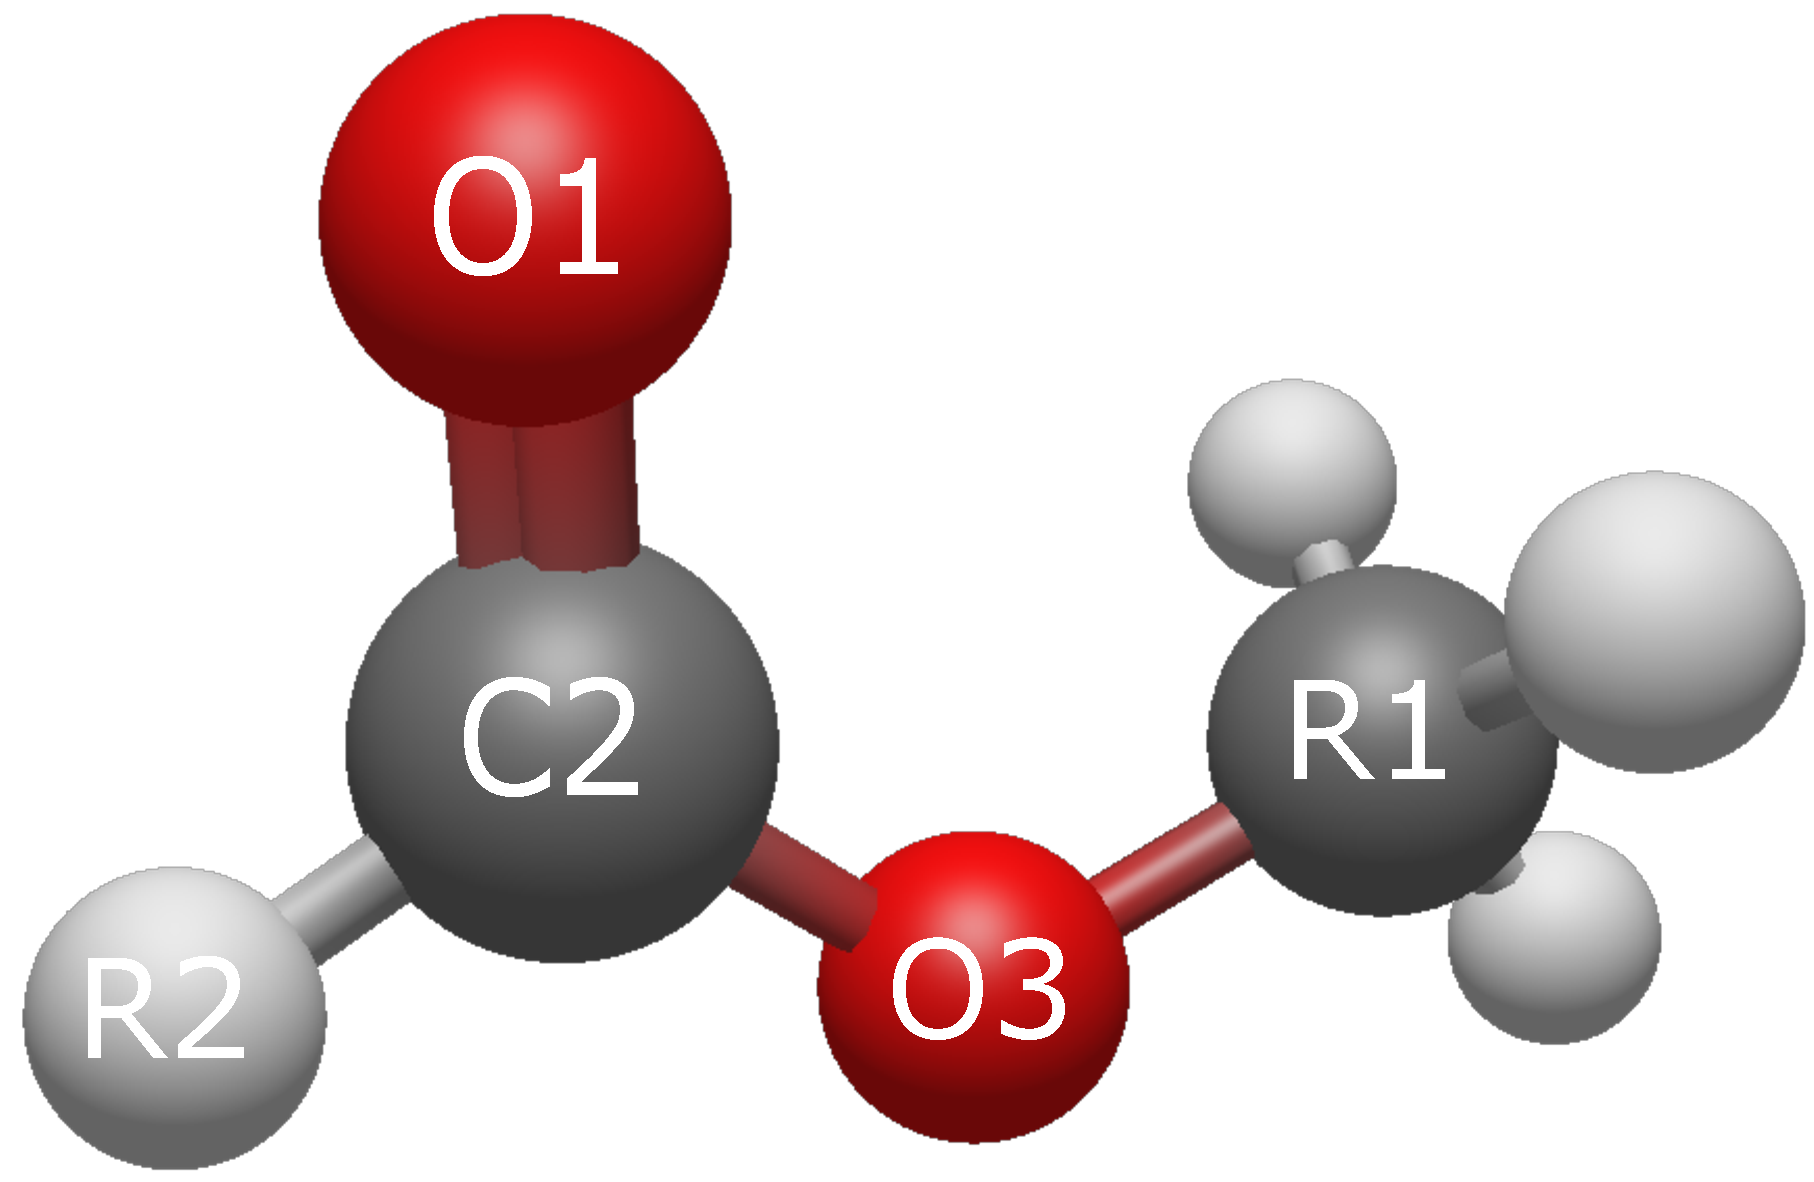
\includegraphics[width=0.4\linewidth]{graphs/methylformate}
		\caption{Esquema de ordenamiento implementado en la matriz Z para los sistemas moleculares bajo estudio: ox\'{i}geno principal (O1), carbono de carbonilo (C2), ox\'{i}geno secundario o adyacente (O3), y sustituyentes (R1 y R2).}
		\label{fig:methylformate}
	\end{figure}

	\clearpage

		\tikzset{
			estiloAzul/.style={
				rectangle, rounded corners=4pt,
				draw=blue!60!black, fill=blue!8,
				text width=4.5cm, align=center,
				minimum height=1.5cm, font=\small,
				drop shadow
			},
			estiloNaranja/.style={
				rectangle, rounded corners=4pt,
				draw=orange!70!black, fill=orange!8,
				text width=4.5cm, align=center,
				minimum height=1.5cm, font=\small,
				drop shadow
			},
			estiloTeal/.style={
				rectangle, rounded corners=4pt,
				draw=teal!60!black, fill=teal!10,
				text width=4.5cm, align=center,
				minimum height=1.5cm, font=\small,
				drop shadow
			},
			estiloVerde/.style={
				rectangle, rounded corners=4pt,
				draw=yellow!50!black, fill=yellow!15,
				text width=4.5cm, align=center,
				minimum height=1.5cm, font=\small,
				drop shadow
			},
			estiloMorado/.style={
				rectangle, rounded corners=4pt,
				draw=purple!60!black, fill=purple!8,
				text width=4.5cm, align=center,
				minimum height=1.5cm, font=\small,
				drop shadow
			},
			estiloFinal/.style={
				rectangle, rounded corners=4pt,
				draw=green!50!black, fill=green!12,
				text width=4.5cm, align=center,
				minimum height=1.5cm, font=\small,
				drop shadow
			},
			flechaModerna/.style={-{Stealth[length=2.5mm]}, thick, black}
		}
		
		\begin{figure}[htbp!]
			\centering
			\scalebox{0.70}{
				\begin{tikzpicture}[node distance=1.5cm and 1.2cm]
					
					% Fila superior (1 -> 2 -> 3)
					\node (start) [estiloAzul] {1. Selecci\'{o}n de datos \\ Obtenci\'{o}n de estructuras de \'{e}steres en PubChem.};
					
					\node (p1) [estiloNaranja, right=of start] 
					{2. Reordenamiento at\'{o}mico \\ Establecer el patron O1, C2, O3, R1 y R2.};
					
					\node (p2) [estiloTeal, right=of p1] 
					{3. Generaci\'{o}n de matrices Z \\ Conversi\'{o}n de coordenadas cartesianas a coordenadas internas.};
					
					% Fila inferior (4 -> 5 -> 6)
					\node (calc) [estiloVerde, below=of p2] 
					{4. C\'{a}lculos mecanocu\'{a}nticos \\ Optimizaci\'{o}n de estructuras $\omega$B97X-D/cc-pVDZ, CPCM.};
					
					\node (aplica) [estiloMorado, left=of calc] 
					{5. An\'{a}lisis de frecuencias \\ Verificaci\'{o}n de un m\'{i}nimo en la superficie de energ\'{i}a potencial.};
					
					\node (end) [estiloFinal, left=of aplica] {6. Obtenci\'{o}n de funci\'{o}n extendida (WFX).};
					
					% Flechas
					\draw [flechaModerna] (start) -- (p1);
					\draw [flechaModerna] (p1) -- (p2);
					\draw [flechaModerna] (p2) -- (calc);
					\draw [flechaModerna] (calc) -- (aplica);
					\draw [flechaModerna] (aplica) -- (end);
					
				\end{tikzpicture}
			}
			\caption{Protocolo computacional para la preparaci\'{o}n, optimizaci\'{o}n y obtenci\'{o}n de la funci\'{o}n de onda extendida (WFX) en \'{e}steres.}
			\label{fig:Potocolo}
		\end{figure}

	
		Una vez reordenadas las coordenadas cartesianas, estas son transformadas en matrices Z, las cuales sirven como geometr\'{i}as de entrada para c\'{a}lculos mecanocu\'{a}nticos. Las optimizaciones de las geometr\'{i}as y los c\'{a}lculos de frecuencias vibracionales son realizadas en \textit{Gaussian09} \citeonline{g09}. Respecto al nivel de teor\'{i}a, se emplea un funcional de la densidad con correcciones de dispersi\'{o}n conocido como $\omega$B97X-D, ya que este nivel de teor\'{i}a exhibi\'{o} una alta correlación ($R^2$ = 0.9680) reportada por \cite{Caballero-Garcia2019} en combinaci\'{o}n con la base de funciones de correlaci\'{o}n consistente cc-pVDZ. Adem\'{a}s, para garantizar la localizaci\'{o}n de un m\'{i}nimo de energ\'{i}a en la superficie de energ\'{i}a potencial y descartar posibles estados de transici\'{o}n, se realiza un an\'{a}lisis de frecuencias. Asimismo, las simulaciones se llevan a cabo considerando los efectos de solvataci\'{o}n impl\'{i}cita en agua, empleando el modelo continuo de polarizaci\'{o}n conductor (CPCM) y se implementa una rejilla de integraci\'{o}n ultrafina (integral=grid=ultrafine) para mejorar la precisi\'{o}n num\'{e}rica de las integrales de intercambio y correlaci\'{o}n. Finalmente, se configura cada mol\'{e}cula para generar de manera directa la informaci\'{o}n de las funciones de onda extendida, las cuales servir\'{a}n como pilares fundamentales para el an\'{a}lisis posterior e interpretaci\'{o}n de la densidad electr\'{o}nica y otras propiedades derivadas de esta.
		
	\clearpage
	
	\section{Perspectivas de trabajo}
	
	La implementaci\'{o}n computacional descrita anteriormente permitir\'{a} establecer un flujo de trabajo sistem\'{a}tico y reproducible para el an\'{a}lisis del grupo carbonilo. A trav\'{e}s de la estandarizaci\'{o}n de las matrices Z y la posterior optimizaci\'{o}n de la geometr\'{i}a al nivel de teor\'{i}a $\omega$B97X-D/cc-pVDZ, se prev\'{e} la obtenci\'{o}n de estructuras moleculares que simulen condiciones fisiol\'{o}gicas o acuosas mediante el modelo CPCM. Adem\'{a}s, la generaci\'{o}n de las funciones de onda extendida constituye la base de este proyecto, pues se espera que dicha informaci\'{o}n permita mapear de forma detallada la densidad electr\'{o}nica de los sistemas estudiados mediante el software propio \textit{DensToolKit2} \cite{Solano2024}.
		
		\clearpage
	%****************************************************************************
	\section{Cronograma de actividades}
	%****************************************************************************
	
	\begin{table}[hbp!]
		\centering
		\footnotesize
		\setlength{\tabcolsep}{8.0pt}
		\begin{tabular}{||p{0.6\linewidth}|c|c|c|c|c|c|c|c|}
			\hline
			\multirow{2}{*}{\centering\textbf{Actividad}} & \multicolumn{8}{c|}{\textbf{Semestre}}\\
			& 1 & 2 & 3 & 4 & 5 & 6 & 7 & 8\\\hline\hline
			Revisi\'{o}n bibliogr\'{a}fica & x  & x & x  & x & x  & x & x  & x\\ \hline
			Curso optativo 1 (reactividad qu\'{i}mica) & x & &&&&&&\\ \hline
			Selecci\'{o}n de sistemas de estudio & x & &&&&&&\\ \hline
			Selecci\'{o}n de programas de c\'{o}mputo & x & &&&&&&\\ \hline
			%
			Curso optativo 2 (m\'{e}todos de la qu\'{i}mica cu\'{a}ntica) &  & x&&&&&&\\ \hline
			C\'{a}lculos principales &x&x&x&x&x&x&&\\ \hline
			Asistencia a congreso nacional (RMFQT) &&&x&&x&&x&\\ \hline
			Examen predoctoral &  & &&x&&&&\\ \hline
			%Escritura de art\'{i}culo &  & &&&x&x&&\\ \hline
			Env\'{i}o y revisi\'{o}n de art\'{i}culo &  & &&&&x&x&\\ \hline
			Asistencia a congreso internacional &  & & & &&x&&\\ \hline
			Escritura de tesis & &&&&&x&x&x \\ \hline
			%Escritura de segundo art\'{i}culo &&&&&&&x&\\ \hline
			Redacc\'{o}n de segundo art\'{i}culo &  & &&&&&&x\\ \hline
			Presentaci\'{o}n del examen profesional & &&&&&&&x \\
			\hline
		\end{tabular}
	\end{table}
	
	
	\newpage
	
	
	\bibliographystyle{ieeetr}   
	\bibliography{bibliografia.bib}   % name your BibTeX data base

	\end{document}  
	
	%%%%%%%%%%%%%%%%%%%%%%%%%%%%%%%%%%%%%%%%%%%%%%%%%%%%%%%%%%%%%%%%%%%%%%%%%%%%%%%%%%
\end{document}
%%%%%%%%%%%%%%%%%%%%%%%%%%%%%%%%%%%%%%%%%%%%%%%%%%%%%%%%%%%%%%%%%%%%%%%%%%%%%%%%%


Comentar que se tienen todas los wfxs.

Utilizar diferentes conf\'{o}rmeros y utilizar promedios ponderados.
